\chapter{Risk Management Framework}
\label{chap:risk_management}

This chapter presents the basic components of GreenGrid Energy's information security risk management programme. It outlines the Risk Assessment Policy, the Risk Assessment and Treatment Processes, and includes an Asset Inventory developed in accordance with ISO/IEC 27001 Clause 6.1.2 and Annex A 5.9.

\section{Risk Assessment Policy}
\label{sec:risk_policy}

\subsection*{Purpose and Scope}
This policy defines GreenGrid Energy's approach to identifying, assessing and managing information security risks. It applies to all information systems, assets, business processes and personnel within the scope of the \ac{ISMS}.

\subsection*{Objectives}
\begin{itemize}
    \item Establish a structured and repeatable approach to risk identification and analysis.
    \item Support informed decision making regarding the implementation of security controls.
    \item Ensure compliance with applicable legal, regulatory and contractual requirements.
\end{itemize}

\subsection*{Governance and Risk Appetite}
\label{subsubsection:risk_apetite}

GreenGrid Energy maintains a conservative risk appetite, particularly for critical infrastructure such as \ac{SCADA} systems and sensitive customer information. Risks rated \textit{High} or \textit{Medium-High} require mandatory treatment and cannot be accepted without mitigation.

%───────────────────────────────────────────────────────────────────────────────
\section{Risk-Assessment Process}
\label{sec:risk_assessment}
%───────────────────────────────────────────────────────────────────────────────

\subsection*{Process Overview}

GreenGrid Energy evaluates information-security risk through a concise,
four-step loop that is repeated whenever assets, threats or the business
context change:

\begin{enumerate}
  \item \textbf{Identify} – catalogue each asset, its owner, and all credible
        threats \& vulnerabilities.
  \item \textbf{Analyse} – assign a qualitative \emph{Likelihood} and
        \emph{Impact} value to every threat scenario.
  \item \textbf{Evaluate} – calculate the scenario \emph{Criticality} as
        Likelihood~\(\times\)~Impact (Equation~\ref{eq:criticality}) and consult
        the Risk Matrix (Figure~\ref{figure:risk_matrix}) to obtain the
        qualitative risk level.
  \item \textbf{Treat/Monitor} – decide on mitigation, transfer, acceptance or
        avoidance and track residual risk until it falls within the appetite
        defined in Section~\ref{subsubsection:risk_apetite}.
\end{enumerate}

\begin{equation}
  \text{Criticality} = \text{Likelihood} \times \text{Impact}
  \label{eq:criticality}
\end{equation}

\subsection*{Qualitative Scales}

\paragraph{Likelihood}
\begin{itemize}
  \item \textbf{Very Likely} – expected within 12 months.
  \item \textbf{Likely} – plausible in 1–3 years.
  \item \textbf{Possible} – credible but uncommon; 3–5 year horizon.
  \item \textbf{Unlikely} – conceivable once in 5–10 years.
  \item \textbf{Very Unlikely} – practically improbable (\(>\)10 years).
\end{itemize}

\paragraph{Impact}
\begin{itemize}
  \item \textbf{Severe} – prolonged outage (\(>\)48 h), safety/environmental
        harm or regulatory breach.
  \item \textbf{Significant} – major financial loss or customer outage 8–48 h.
  \item \textbf{Moderate} – noticeable service impact 1–8 h, limited legal or
        financial exposure.
  \item \textbf{Minor} – localised disruption, quickly reversible.
  \item \textbf{Negligible} – no meaningful effect on operations or reputation.
\end{itemize}

\begin{figure}[H]
  \centering
  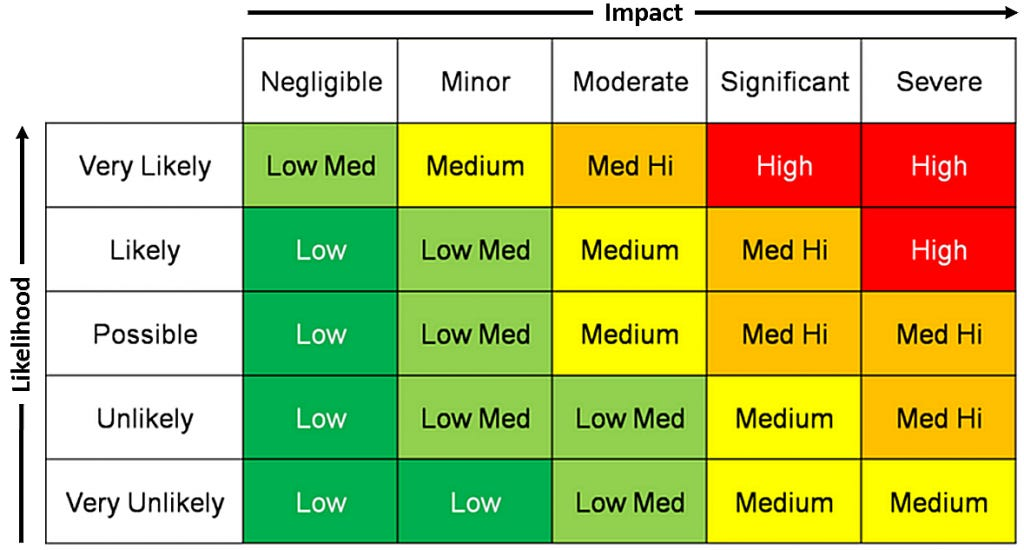
\includegraphics[width=0.85\textwidth]{figures/image.png}
  \caption{GreenGrid Energy qualitative 5 × 5 risk matrix.}
  \label{figure:risk_matrix}
\end{figure}

The matrix yields one of five qualitative results—\textbf{High},
\textbf{Medium-High}, \textbf{Medium}, \textbf{Low-Medium} or \textbf{Low}.
Any scenario that registers as \textbf{High} or \textbf{Medium-High} exceeds
the organisation’s risk appetite and must enter the treatment workflow
immediately.

\subsection*{Accountability}
\label{subsec:risk_ownership}

\begin{itemize}
  \item \textbf{Asset Owner} – maintains the asset record, validates the
        Likelihood/Impact assignment, funds the chosen treatment and signs off
        any residual risk that is to be accepted.
  \item \textbf{Information Security Manager (ISM)} – supplies the methodology,
        moderates scoring for consistency and escalates overdue High or
        Medium-High risks to the Risk Committee.
  \item \textbf{Risk Committee} – reviews and approves residual risks at
        Medium-High or above and arbitrates conflicts between operational needs
        and risk-reduction actions.
\end{itemize}

These role assignments place day-to-day responsibility with the people closest
to each asset while providing clear organisational oversight and escalation
paths.


\subsection{Risk Identification}

\subsubsection{Asset Inventory}

As part of the risk identification process required by ISO/IEC 27001, a complete asset inventory was developed and classified according to security relevance and operational context. This inventory includes both \ac{IT} and \ac{OT} assets and was used as a reference to assess risk levels based on the \ac{CIA} triad.

The full inventory is presented in Appendix~\ref{appendix:asset_inventory}, where assets are organised by department and include detailed technical and risk-related attributes.

\subsection{Risk Analysis}

Following the identification of relevant assets and their classification according to Confidentiality, Integrity, and Availability (CIA), a structured risk analysis was performed. This process involved evaluating the likelihood and potential impact of various threat scenarios targeting the organisation’s information assets.

The methodology applied is based on a qualitative risk matrix approach, combining the likelihood of occurrence with the impact level to determine the severity of each risk. Likelihood levels were derived from historical incident trends, industry threat intelligence, and system exposure (e.g., public-facing interfaces or outdated software). Impact levels were assessed considering the potential consequences on operations, legal compliance, financial stability, and reputation.

The risk matrix used by GreenGrid Energy, shown in Figure~\ref{figure:risk_matrix}, categorises risks into four levels: Low, Medium, High, and Critical. These categories support the prioritisation of treatment measures in the subsequent phase.

\subsection{Risk Assessment}

The risk assessment stage consists of comparing the analysed risk levels with GreenGrid Energy’s defined risk acceptance criteria. Risks classified as High or Critical are considered unacceptable and require mandatory treatment through mitigation, transference, or avoidance. Medium-level risks may be tolerated if justified and documented with compensatory controls or a monitoring strategy. Low-level risks are generally accepted, but still logged for periodic review.

Each identified risk was documented with:
\begin{itemize}
    \item Affected asset and department;
    \item Identified threat or vulnerability;
    \item Likelihood and impact rating;
    \item Calculated risk level (from the matrix);
    \item Proposed treatment or justification for acceptance.
\end{itemize}

The outcome of the risk assessment provides the foundation for the selection and implementation of appropriate security controls, ensuring alignment with both ISO/IEC 27001 and GreenGrid Energy’s operational needs and risk appetite.


\section{Risk Treatment Process}
\label{sec:risk_treatment}

\subsection*{Treatment Options}
Risks that exceed acceptable thresholds shall be managed using one or more of the following strategies:
\begin{itemize}
    \item \textbf{Mitigation}: Implementing controls to reduce the likelihood or impact of the risk.
    \item \textbf{Acceptance}: Accepting the risk when its impact is negligible or mitigation is not cost effective.
    \item \textbf{Transference}: To transfer the risk to a third party (e.g. by insurance or outsourcing).
    \item \textbf{Avoidance}: Elimination of the risk by cessation of the associated activity.
\end{itemize}

GreenGrid Energy follows the treatment approach outlined below:
\begin{itemize}
    \item \textbf{High and Medium-High risks} must be mitigated. If mitigation is not possible internally, the risk will be transferred to a competent third party for resolution.
    \item \textbf{Medium risks} will be transferred to qualified external entities for management.
    \item \textbf{Low and low-medium risks} are generally accepted. However, treatment may be considered if there are no higher priority risks pending.
\end{itemize}

\subsection*{Implementation}
A formal plan shall be developed for each risk requiring treatment, including
\begin{itemize}
    \item The chosen management strategy.
    \item Designated stakeholders responsible for implementation.
    \item Implementation schedules and defined monitoring mechanisms.
\end{itemize}


